\chapter{研究背景}
\label{chap:haikei}

本章では手書きメモ・イラストを扱う既存のシステムの現状と、その問題点を整理する。

\newpage

\section{手書きのメモ・イラスト}
手書きによるメモやイラストは情報を記録・表現する手法として広く普及している。
筆記具と紙さえあればすぐに記録でき、また美麗な作品を描くことを目的としなければ、特別な技量も要求されないためである。
計算機の登場によりテキスト編集支援機能が充実したため、文章のみで完結する内容であれば手書きではなくテキストとして記録するように置き換わったが、
アイデアのような文章のみでは表現しづらい構造を持った概念を表現する場合は文字と図を自在に混合させて配置できる手書きメモの方が適している。
また、テキストによってメモをとる場合はキーボードのような専用のハードウェアや、それらを使いこなすタッチタイピング等の技量が必要であるという問題点があるが、
手書きの場合は紙やペン等の筆記具が扱えれば良いため、ハードウェアや技能を必要とするテキスト入力と比較してより多くの人々が利用できる手段であると言える。

\section{タッチ・ペンインターフェースの普及}

\begin{figure}[htbp] \begin{minipage}{0.5\hsize}
                         \begin{center} {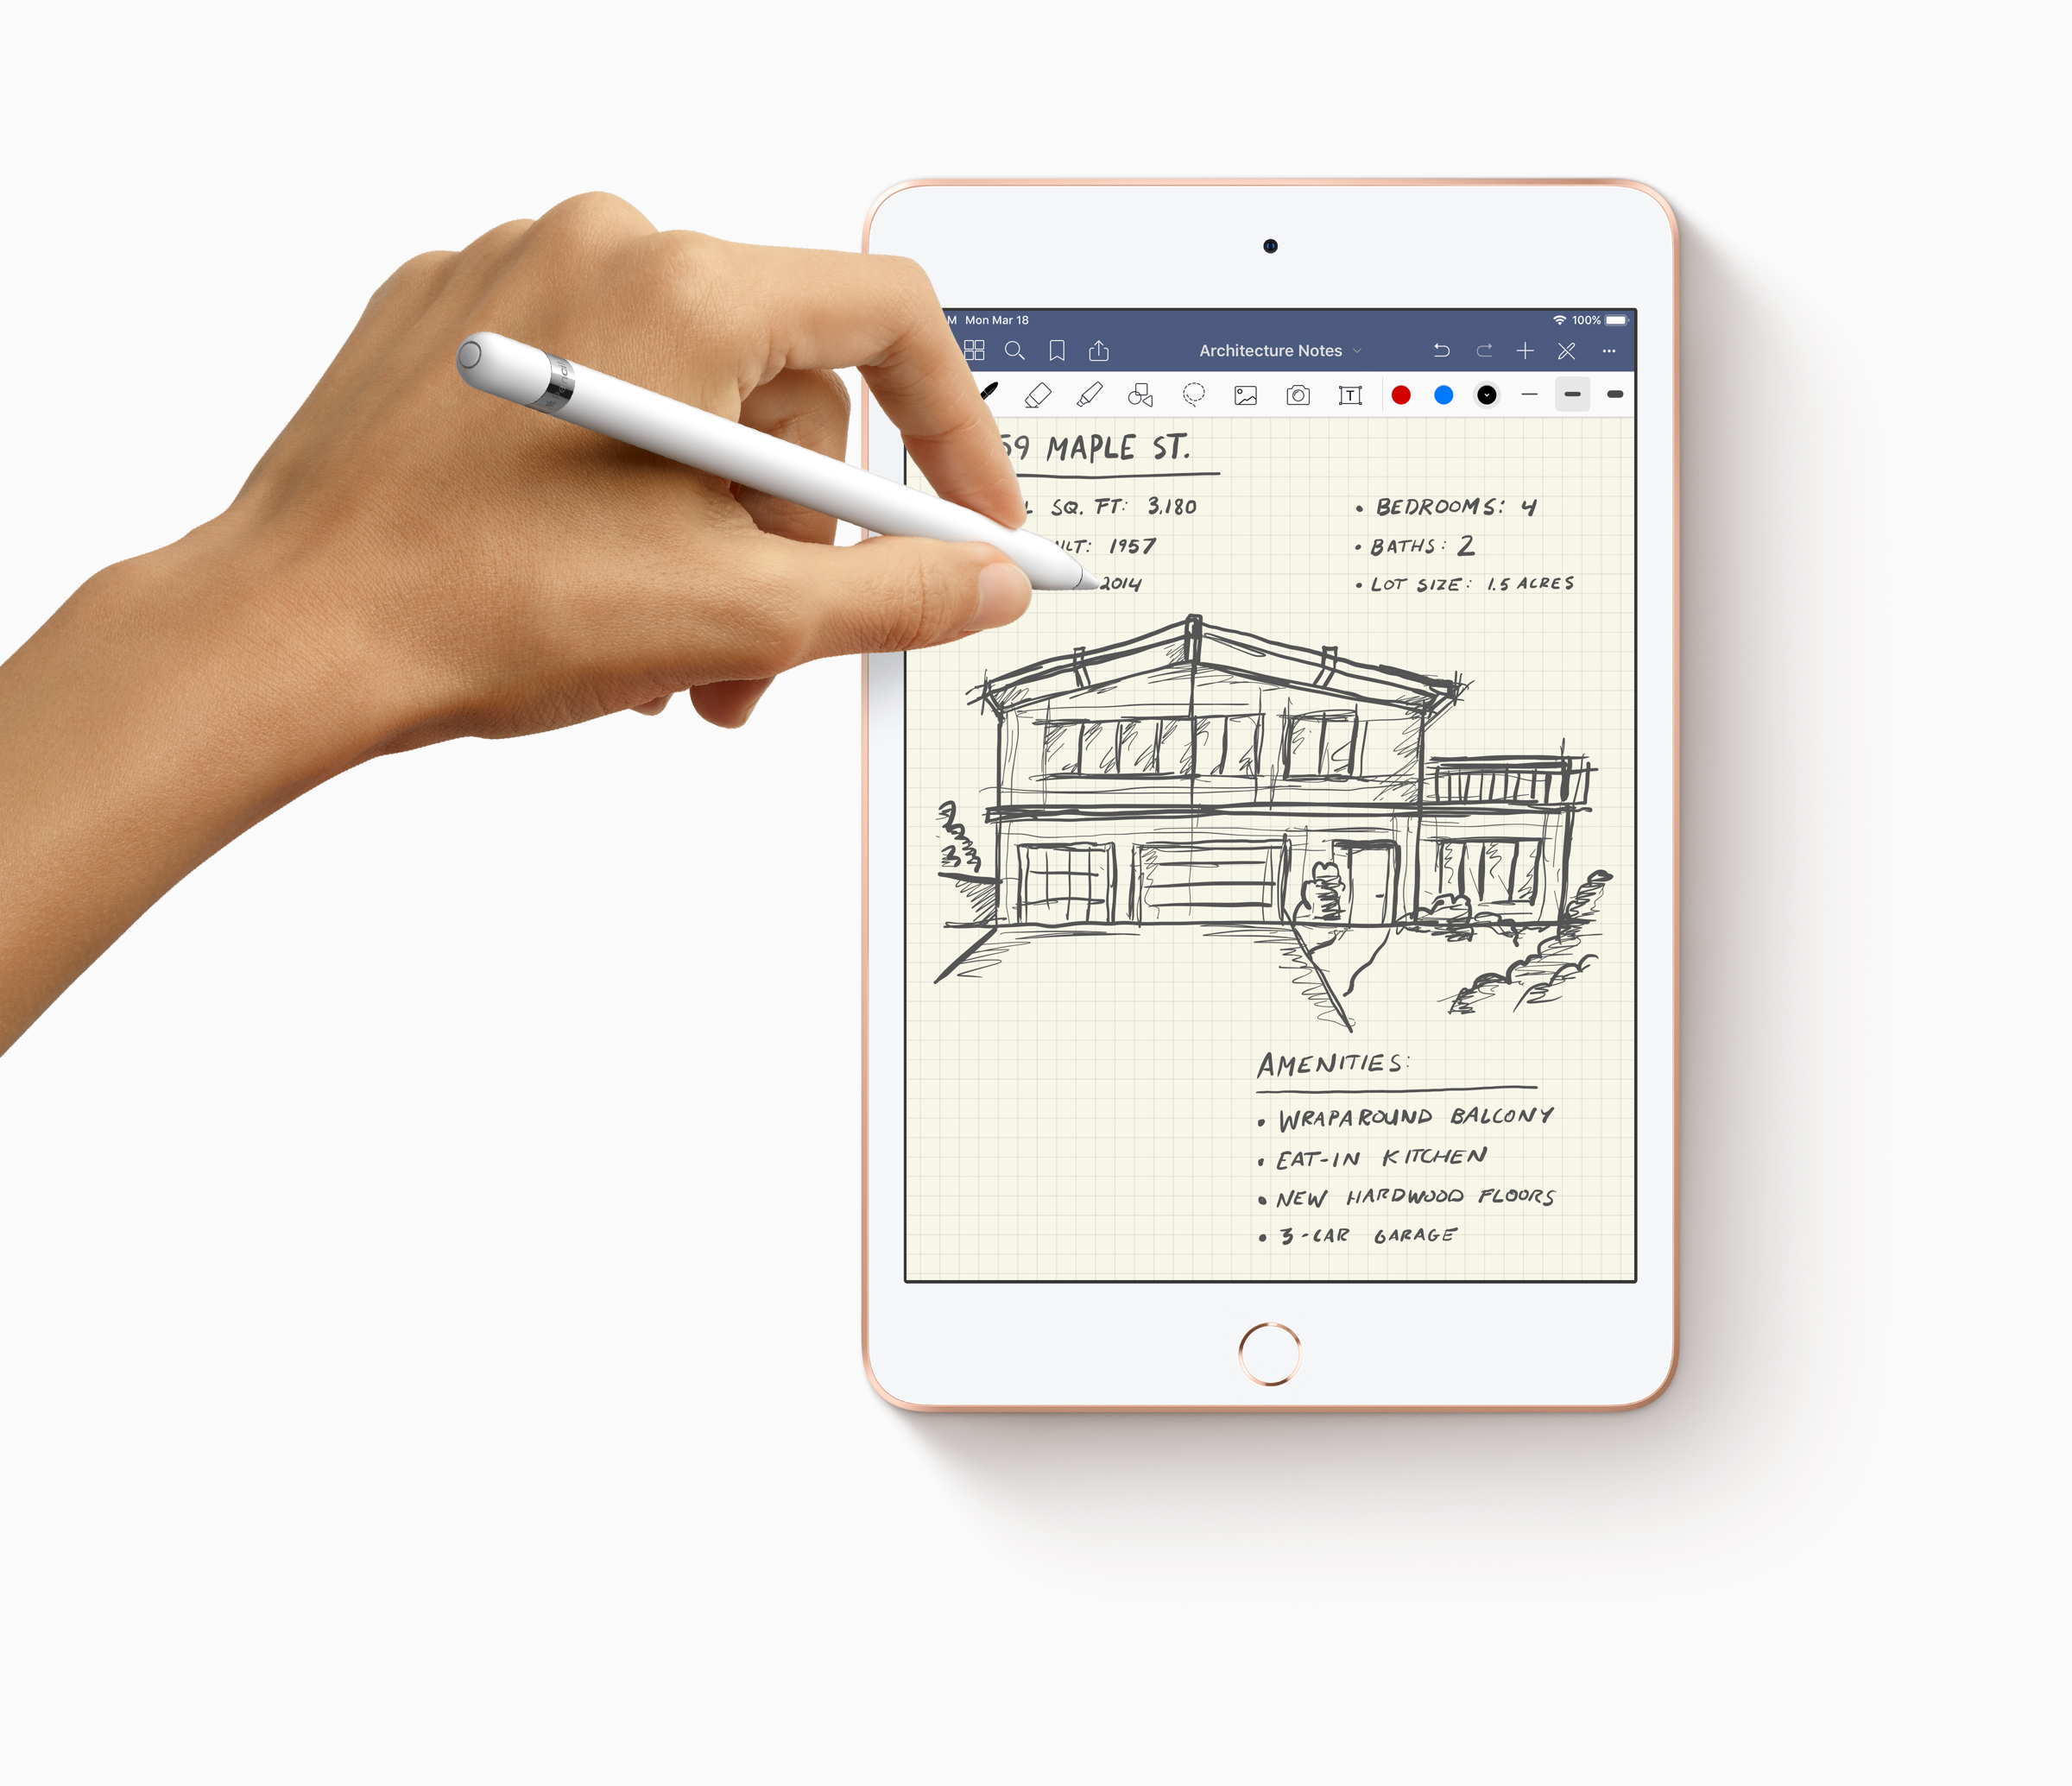
\includegraphics[width=40mm]{images/ipadmini.jpg}}
                         \end{center} \caption{iPad}
\end{minipage} \begin{minipage}{0.5\hsize}
                   \begin{center} {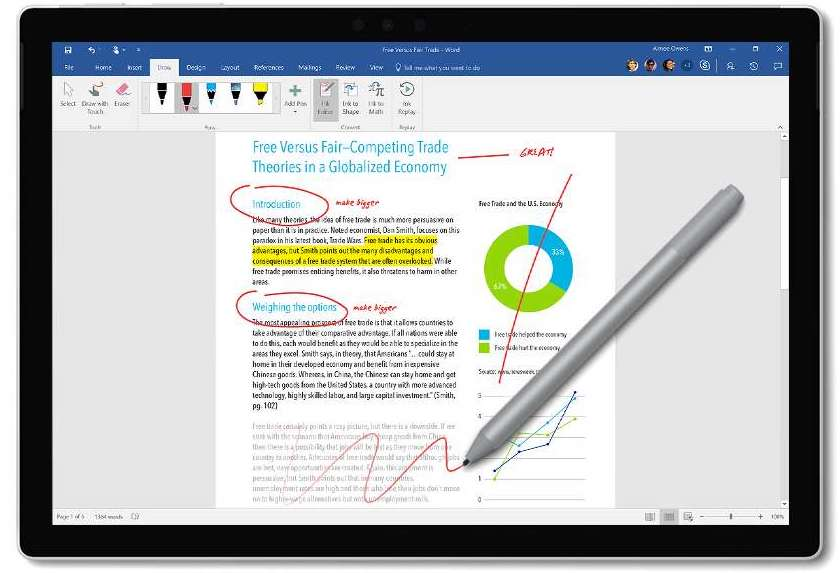
\includegraphics[width=40mm]{images/surface.jpg}}
                   \end{center} \caption{Surface}
\end{minipage}
\end{figure}

かつてはノートやスケッチブック等の紙の上で記録されていた手書きメモだが、タッチパネルやスタイラスペン等のインターフェースを備えたデバイスの普及に伴い、
計算機上で手書きメモを取ることが一般化してきた。
手書きメモやイラストを計算機の上で描く場合、マウスやトラックパッド等のポインティングデバイスではなく、
スタイラス等のペンインターフェースが好ましいとされるが、iOS\footnote{https://www.apple.com/jp/ios/}やWindows\footnote{https://www.microsoft.com/ja-jp/windows}、
ChromeOS\footnote{https://www.google.com/chromebook/}等の主要なプラットフォームで
スタイラスペンを備えた機種が充実しているため手書きでメモやイラストを描く環境は充分に整っていると考えられる。

\section{計算機上で手書きメモ・イラストの作成支援}
計算機上でメモやイラストを作成する場合、以下のような編集支援機能を利用することができる。
\begin{itemize}
    \item コピーやペースト
    \item UndoやRedo
    \item オブジェクトの移動や変形
\end{itemize}
これらの機能は紙という物理的なメディアの上では実現不可能であったが、現在では手書きデータを扱う大抵のアプリケーションが備えている。
計算機の進化によって、手書きメモ・イラストの作成については編集支援機能によって利便性が大きく向上したと言える。

\section{手書きデータを表現する画像ファイルフォーマットの制約}
一方で作成した手書きメモを保存・記録する画像ファイルのフォーマットの機能は大きく制限されている。
一般的に出力先としてJPEGやPNG等のビットマップ画像が用いられているが、この種のフォーマットは描いたもの全てがピクセルの集合として統合・変換されるため、
インクをピクセルに置き換えただけのファイルとして保存される。
したがって画像ファイルを参照するためには、
\begin{itemize}
    \item 命名規則に則ってファイル名を決める
    \item 階層構造を設定してフォルダ分けする
    \item タグを複数設定してファイルにラベリングする
\end{itemize}
等の管理・運用上の工夫が必要となる。
手書きメモを計算機で作成することは可能になったが、その参照や管理の不便さ、再利用の難しさは
紙の上でメモをとっていたころからあまり改善されていない。


\section{手書きメモ・イラストを扱う既存のシステム}

\subsection{メモアプリケーション}
手書きデータを効率よくメモとして扱うことを目的とするシステムを解説する。

\subsubsection{iOS/Macのメモアプリ}

\begin{figure}[htbp]
    \begin{center}
%        \fbox {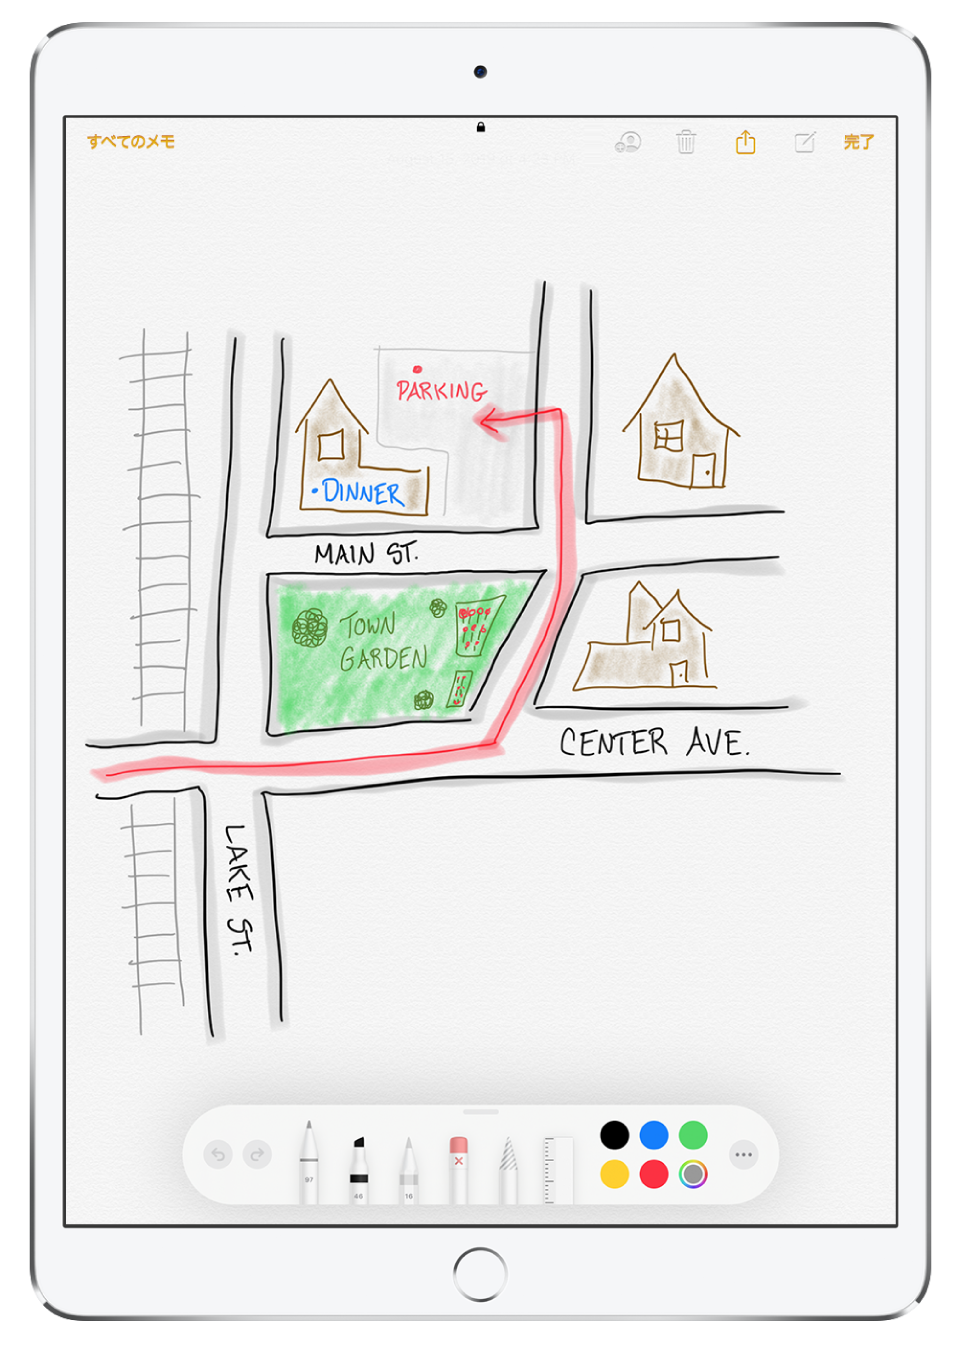
\includegraphics[width=50mm]{images/applememo.png}} \end{center}
        \fbox {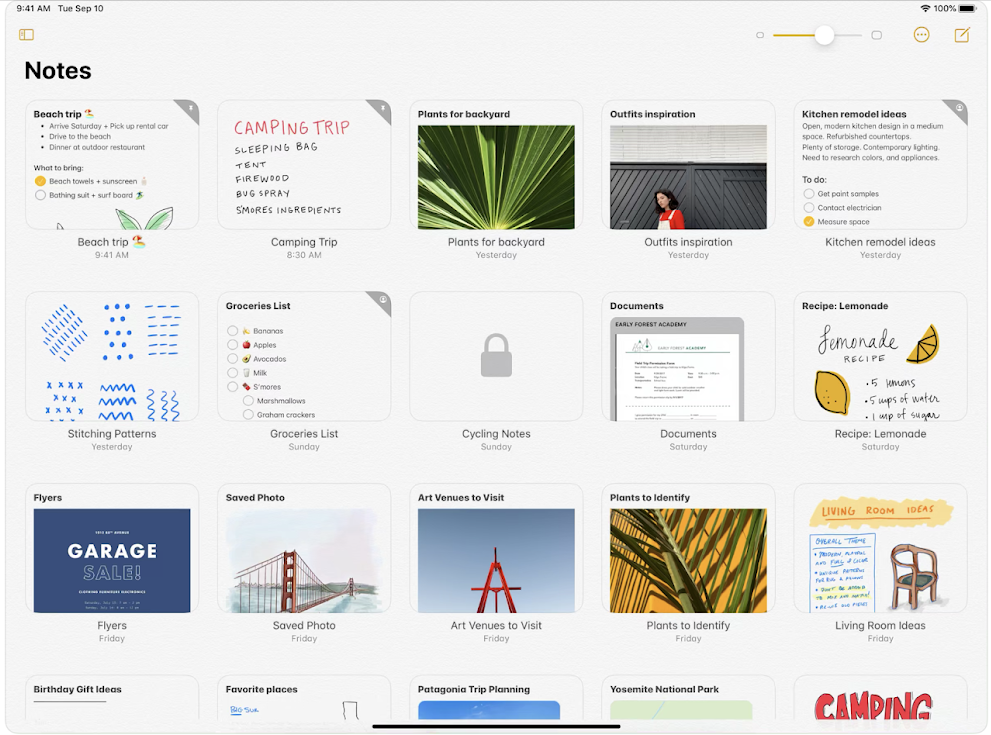
\includegraphics[width=80mm]{images/iosmemo.png}} \end{center}
    \caption{iOSのメモ}
\end{figure}

AppleのiPadやMacにはメモアプリケーションが標準でインストールされており、指やApple Pencilを用いて素早く手書きメモを取ることができる。
一方で描いた手書きメモは画像として保存されるのみで、それを後から検索する機能は存在しないため、参照できるように
ファイル名を決める、もしくは保存するフォルダを分類する等の工夫が求められる。

\subsubsection{Evernote}

Evernote Corporationが開発するEvernoteは指やスタイラスペンで手書きのメモやスケッチを作成できるほか、
手書きメモ内の文字を認識し、全文検索によって手書きメモを参照する機能を備えている。
あくまで検索対象は認識できた手書き文字のみであり、図形や描いたものの形状等のグラフィカルなデータから手書きメモを参照することはできない。
そもそもEvernoteにおいて手書きメモを含めた全てのメモはノートブックと呼ばれる階層に分類して管理することを前提としているため、
今取っているメモはどのノートブックに属するものかを予め意識する必要がある。

\subsubsection{Google Keep}

Googleが開発するGoogle Keepも、Evernoteと同様に手書き文字を認識し、テキスト検索を行う機能を備えている。
Evernoteと異なり、Google Keepにはフォルダ等の階層構造はなく、全てのメモがフラットに管理される。
必要に応じてメモに色やラベルをつけることによって、複数のメモを分類できるようデザインされている。

\begin{figure}[htbp] \begin{minipage}{0.5\hsize}
                         \begin{center} \fbox {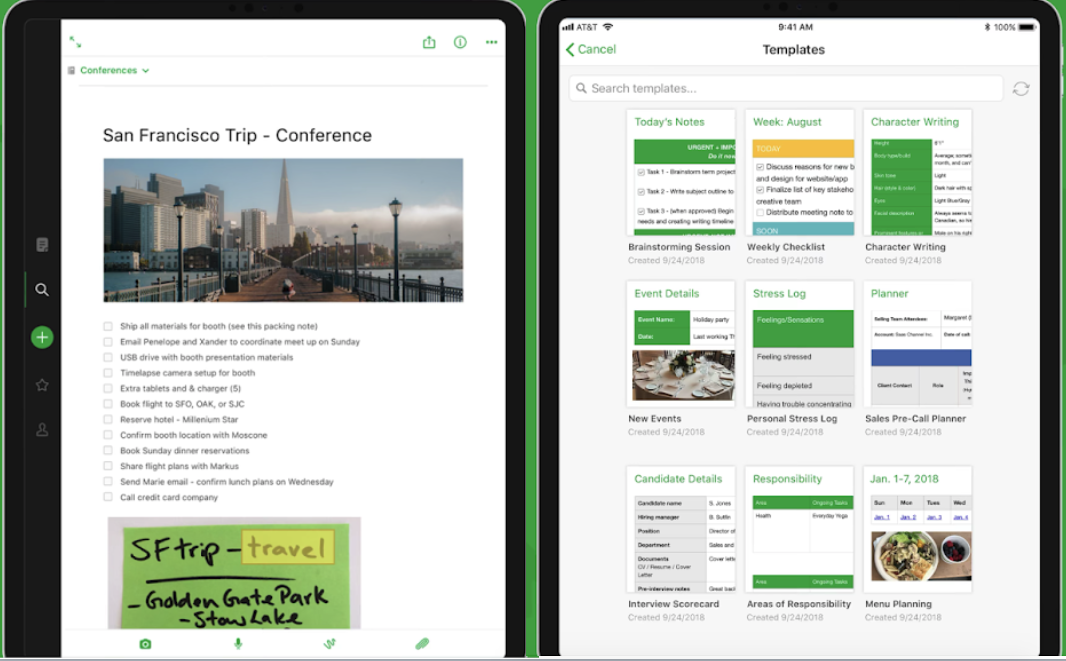
\includegraphics[width=70mm]{images/margedevernote.png}}
                         \end{center} \caption{evernote} \label{fig:evernote}
\end{minipage} \begin{minipage}{0.5\hsize}
                   \begin{center} \fbox {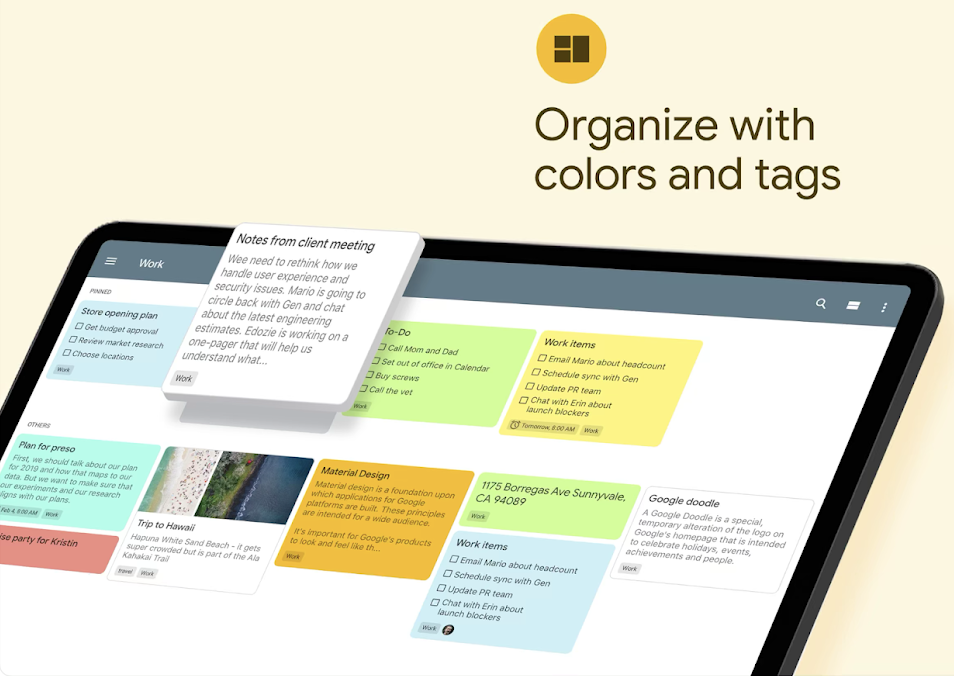
\includegraphics[width=70mm]{images/iosgooglekeep.png}}
                   \end{center} \caption{googlekeep} \label{fig:googlekeep}
\end{minipage}
\end{figure}

\subsection{イラスト投稿・共有システム}
Web上に投稿・共有されたイラストを、効率よく参照できるよう管理することを目的としたシステムを解説する。
これらのシステムは基本的に完成されたアート作品を投稿するのが主な用途であり、メモを素早く記録する手段
として使われることはない。

\section{テキストの進化}
手書きのメモやイラストと同様に紙の上で記録されていたテキストは計算機の登場により以下のような機能を獲得した。
\begin{itemize}
    \item 編集支援機能\\
    コピーやペースト、UndoやRedo等の便利な機能によって簡単に文章が書けるようになった。
    \item ハイパーリンク\\
    異なる文書への参照をハイパーリンクによって記述でき、素早く関連文書を参照できるようになった。
    \item ハイパーテキスト\\
    ハイパーリンクやマルチメディアを埋め込めるハイパーテキストの登場で、よりリッチなコンテンツを作成できるようになった。
\end{itemize}
これにより参照・管理・再利用が難しいという問題点が解決されただけでなく、新しい活用法が発明されることとなった。

\subsection{Wikiシステム}

wardらにより開発されたWiki\cite{Leuf2001TheWW}は ハイパーリンクやマルチメディアを含んだハイパーテキストを
手軽に作成・編集できるインターフェースを備えたアプリケーションである。
複数人が共同で編集することも可能なのでコラボレーションツールとしても活用することができる。
Wikipedia\footnote{https://www.wikipedia.org/}はよく知られたWikiの実装例の一つである。

\subsubsection{Scrapbox}
Scrapbox\footnote{http://scrapbox.io/}はGyazz\cite{Gyazz}をベースに開発され、Nota\footnote{\textsf{https://www.notainc.com/ja}}社よって運営されている
Wikiシステムで、他のシステムには無い以下のような特徴的な機能を備えている。
\begin{itemize}
    \item シンプルな記法とWYSIWYGエディタ\\
        Scrapboxではページ間のリンクや、外部リンクを含んだ画像や動画、音声等のメディアを
        \texttt{[]}を基本としたシンプルな記法で記述することができる。

    \item 関連ページの表示機能\\
        Scrapboxではページの下部に
        \begin{itemize}
                  \item 別ページへのリンク
                  \item 別ページからのリンク
                  \item リンク先ページがリンクしているページ
        \end{itemize}等のリンクに基づいた関連ページを表示する機能を備えている。
        Scrapboxにおいてコンテンツとなるページは全てフラットに扱われるが、
        ページ間リンクを元に関連する情報が自動的に推薦されるため、管理や分類を気にすることなく
        コンテンツを参照可能な状態にしておくことができる。
\end{itemize}

\begin{figure}[htbp] \begin{minipage}{0.5\hsize}
                         \begin{center} \fbox{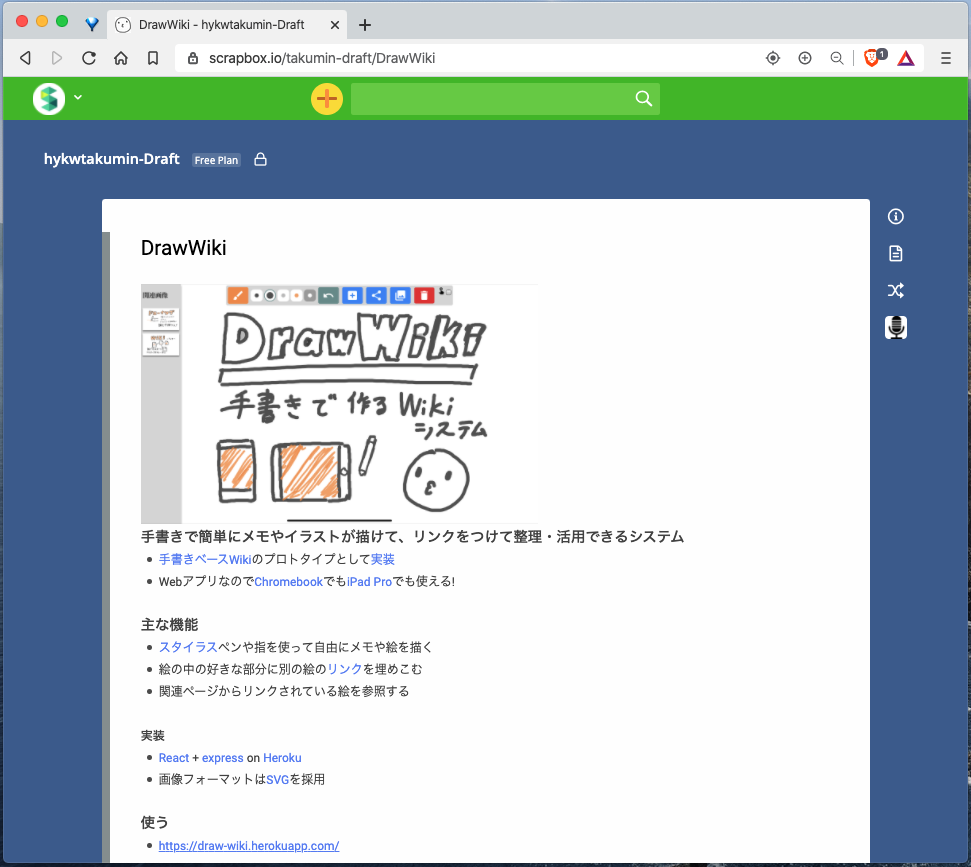
\includegraphics[width=70mm]{images/scrapbox1.png}}
                         \end{center} \caption{Scrapboxの画面} \label{fig:scrapbox1}
\end{minipage} \begin{minipage}{0.5\hsize}
                   \begin{center} \fbox{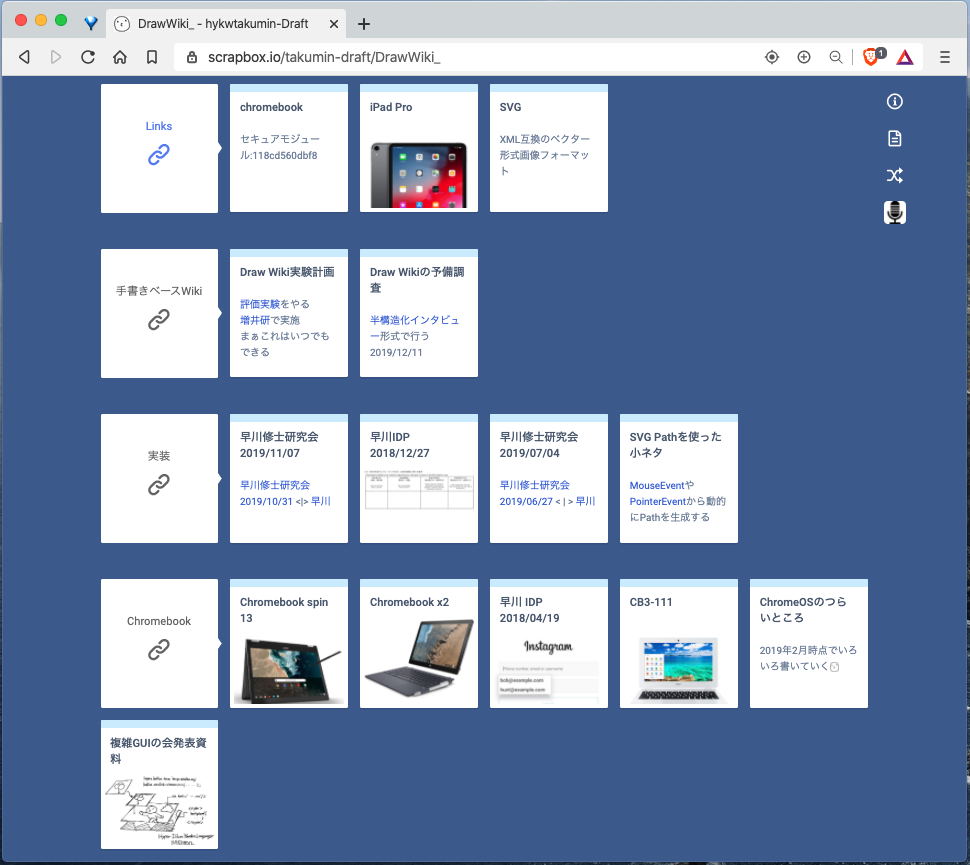
\includegraphics[width=70mm]{images/scrapbox2.png}}
                   \end{center} \caption{関連ページリスト} \label{fig:scrapbox2}
\end{minipage}
\end{figure}

\section{手書きメモ・イラストの問題点}
\label{mondai}
ハイパーテキストとは対照的に手書きメモ・イラストを表現する画像ファイルフォーマットが抱える制約によって、
計算機が普及した現在でも以下のような問題が解決されていない。
\begin{itemize}
    \item 参照や管理が面倒\\
    手書きのメモ・イラストを参照可能な状態にするために、ファイル名や分類先のフォルダやラベリングするタグ等を
    工夫して管理しなければならない。
    \item 再利用が難しい\\
    手書きメモをメモアプリ以外から参照する、別の手書きメモをリンクさせる等の用途が
    既存の手書きメモ・イラストを扱うシステムではそもそも想定されていないため、手書きメモを再利用する
    手段は大きく限定されている。
\end{itemize}


\section{まとめ}
手書きメモ・イラストは広く浸透した情報の記録手法であるものの、紙というフォーマットの制約によって使い勝手が制限されている。
一方で計算機上で手書きメモ・イラストの作成や管理を行うシステムが広く利用されているが、画像ファイルフォーマットの制約から
これらは紙の手書きメモの利用形態を再現したにとどまり、参照や管理、再利用が難しいという本質的な問題は解決されていない。
次章では上記のような問題点を解決するべく、これまでの手書きメモ・イラストの在り方にとらわれない次世代のフォーマット「ハイパーイラスト」と、
それらを容易に管理・再利用できるシステム「手書きベースWiki」を提案する。